\cleardoublepage
\chapter{Preliminaries}

\todo{
Why's the prefix needed for static analysis? => Is it because of the graph representation? (with a prefix, the visibility relation becomes transitive). See the robustness paper. Should we mention what robustness is? Then, the justification for our protocol is that it's the first PSI/NMSI impl amenable to analyse with robustness in mind.\\

Tentative contents:

- ACID vs CAP. What's consistency? What's isolation? What is a consistency guarantee?

- Causal consistency. Vector clocks? Happens-before relationship

- What's a transaction. Follow \textsection 3 in GMU paper

- Explain the different levels of consistency (at least mention RC and SER, so we can talk about them during the evaluation) with the framework presented in Andrea/Alexey's CONCUR'15 paper (A Framework for Transactional Consistency Models with Atomic Visibility), using anomalies and abstract executions.
}

We begin with an introduction to the notation and basic concepts used throughout this thesis. We also review several \emph{strong} and \emph{weak} consistency models, based on the anomalies that are observable in each model. Finally, we discuss several protocols implementing some of these models, representing the previous work against which we compare our approach.

\section{Notation}

In this section, we define the elements we use throughout this chapter, such as transactions, histories, and relations. We follow the models used by Ardekani~\citep{ardekani_thesis}, Adya~\citep{adya_thesis} and Bernstein et al.~\citep{bernstein_concurrency}.

\subsection{Objects and Transactions}

We consider a database storing \textbf{\em objects} $\Obj = \{x, y, \ldots\}$, which we assume to be integer-valued. Clients interact with the database via \textbf{\em transactions} $\Trans = \{\tx_i \mid i \in \mathbb{N}\}$, with $i$ being the \emph{transaction identifier} of $\tx$. A transaction is a totally ordered sequence of read or write operations, followed by a \emph{terminating} operation: either commit or abort. This order follows the order in which the client invoked such operations. Given an object $x$ and a transaction $\tx_i$, we call $x_i$ to the \textbf{\em version} $i$ of $x$ written by $\tx_i$. We denote by $w_i(x_i)$ when a transaction $\tx_i$ writes a version $i$ of $x$, and $r_i(x_i)$ when $\tx_i$ reads a version $i$ of $x$. Finally, we denote by $c_i$ when $\tx_i$ commits, and $a_i$ when it aborts. We assume an initial transaction $\tx_0$ writes the initial versions of every object in the database. Without loss of generality, we also assume that no transaction performs \emph{blind updates}, that is, for every write operation $w_i(x_i)$ performed by $\tx_i$, there's always a preceding read operation $r_i(x_i)$. We say that a transaction is \textbf{\em read-only} if its set of operations does not include writes, and \textbf{\em update} otherwise.

\subsection{Histories}
\label{sect:histories}

We call a \textbf{\em history} $h$ to the finite set of all transactions with disjoint identifiers issued against a database. We denote the set of all possible histories by $\Hist$. For some history $h$, $\hb_h$ denotes a \textbf{\em happens-before} strict partial order over $h$, such that for any two transactions $\tx_i$ and $\tx_j$, if $w_i(x_i)$ and $r_j(x_i)$, $\tx_i \hb_h \tx_j$ (that is, $\tx_j$ reads the version $i$ of $x$ written by $\tx_i$). Intuitively $\tx_i \hb_h \tx_j$ means that $\tx_j$ is aware of the updates performed by $\tx_i$, and thus the outcome of the operations in $\tx_j$ may depend on the effects of $\tx_i$. In this case, we say that $\tx_i$ is a \textbf{\em causal dependency} of $\tx_j$. A transaction $\tx_i$ is \textbf{\em pending} in $h$ if $(c_i \vee a_i) \notin h$. We can represent the history and the relations between operations and transactions as a graph, following Bernstein et al~\citep{bernstein_concurrency}.

\begin{figure}[h]
  \centering
  \vspace{-0.4cm}
  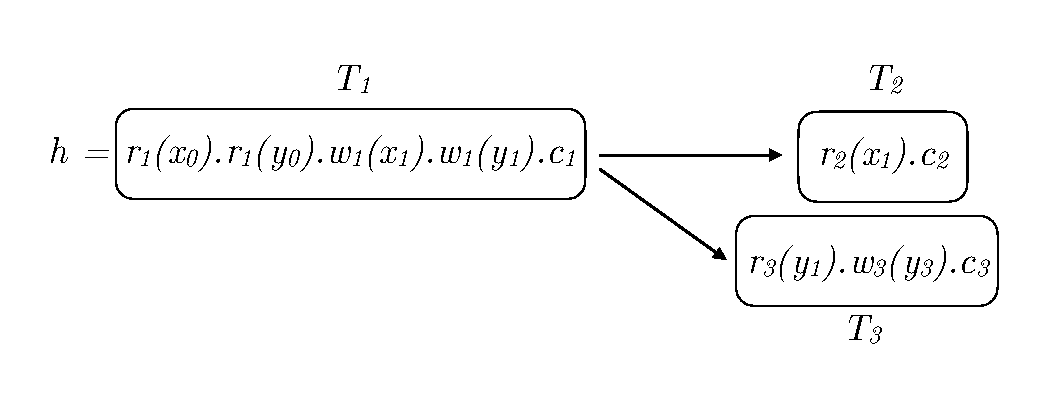
\includegraphics[width=0.7\textwidth]{figures/history.pdf}
  \vspace{-1cm}
  \caption{Example of history represented as a graph. Arrows represent the causal dependencies between operations. Adapted from \em{Ardekani et al.~\citep{ardekani-nsmi}}}
  \label{fig:history}
\end{figure}

Figure~\ref{fig:history} above shows an example, with $\tx_1 \hb_h \tx_3$ and $\tx_1 \hb_h \tx_2$. We say that two transactions $\tx_i$ and $\tx_j$ are \textbf{\em concurrent} in $h$ (denoted by $\tx_i \parallel \tx_j$) if neither $\tx_i \hb_h \tx_j$ nor $\tx_j \hb_h \tx_j$. In the figure above, $\tx_2$ and $\tx_3$ are concurrent.

\section{Consistency Models}

In this section, we define what a consistency model is, distinguishing between \emph{strong} and \emph{weak} models. We give an overview of several models, and compare them in terms of their undesirable effects.

We define a consistency model as a set of histories $\Cons$, such that $\Cons \subseteq \Hist$. Intuitively, a consistency model \emph{constrains} the set of possible histories by specifying how operations interleave in any given history. We say that a given history $h$ \emph{satisfies} a consistency model $\Cons$ if $h \in \Cons$, and that $h$ \emph{violates} $\Cons$.

In the context of databases, the definition of a consistency model maps to the concept of an \emph{isolation level} (I in AC\underline{I}D), which specifies the degree to which concurrent transactions in a database are aware of each other~\citep{adya_thesis}. We use the term consistency throughout this thesis, in accordance with Adya~\citep{adya_thesis}.

Traditionally, the different consistency models have been defined in terms of \emph{anomalies}~\citep{sql-critique}, that map to a set of undesirable histories that are observable by the system. Intuitively, we can distinguish between \emph{strong} and \emph{weak} consistency models depending on the number of anomalies they disallow, with stronger models restricting the set of possible histories more than weak ones. In the sections that follow, we give a brief overview of the traditional anomalies following the definitions advanced by Berenson et al.~\citep{sql-critique}, as well as different consistency models that preclude them. Figure~\ref{fig:anomalies} shows a quick summary of the models and anomalies we cover.

\begin{figure}[h]
\begin{center}
\begin{tabularx}{\linewidth}{ >{\centering}p{8cm} | *{5}{>{\centering}X}}
    \multirow{2}{*}{\em Anomalies} & \multicolumn{5}{c}{Consistency Models} \tabularnewline \cline{2-6}
    & SER & SI & PSI & NMSI & RC \tabularnewline \hline
    Dirty Write & x & x & x & x & x \tabularnewline
    Dirty Read & x & x & x & x & x \tabularnewline
    \hline % Distinguish between ACID or not
    Non-Repeatable Read & x & x & x & x & \checkmark \tabularnewline
    Lost Update & x & x & x & x & \checkmark \tabularnewline
    \hline % Distinguish between weak and strong
    Write Skew & x & \checkmark & \checkmark & \checkmark & \checkmark \tabularnewline
    Long Fork & x & x & \checkmark & \checkmark & \checkmark \tabularnewline
    Non-Monotonic Snapshot & x & x & \checkmark & \checkmark & \checkmark \tabularnewline
\end{tabularx}
\end{center}
\caption{Anomaly Comparison of Consistency Models \emph{(x}:disallowed, \checkmark:allowed\emph{)}. Adapted from \em{Ardekani et al.~\citep{ardekani-nsmi}}}
\label{fig:anomalies}
\end{figure}

\begin{definition}[Dirty Write]
A \emph{Dirty Write} occurs in a history $h$ when a transaction $\tx_i$ modifies an object $x$ that was previously modified by another pending transaction $\tx_j$. If any of the two transactions commit or abort, it is not clear what value the object $x$ should have. A Dirty Write can be represented by a history such as $w_1(x_1).w_2(x_2).(c_1 \vee a_1).(c_2 \vee a_2)$, where the termination order of the transactions can be arbitrary. The anomaly occurs even if any of the transactions aborts.
\end{definition}

\begin{definition}[Dirty Read]
A \emph{Dirty Read} occurs in a history $h$ when a transaction $\tx_i$ reads an object $x$ modified by a pending transaction $\tx_j$. If $\tx_j$ ultimately aborts in $h$, the value observed by a $\tx_i$ was never supposed to occur in $h$. This is represented by a history such as $r_1(x_0)\ldots w_1(x_1)\ldots r_2(x_1)\ldots c_2\ldots a_1$.
\end{definition}

Both of these anomalies can be prevented by making a transaction's changes visible only after it commits. For example, updates can be buffered locally in the context of a transaction. All the consistency models we describe in the sections that follow preclude dirty writes and reads. Transactions executing under such models offer \emph{atomicity} (A in \underline{A}CID).

\begin{definition}[Non-Repeatable Read]
A non-repeatable read---also called a \emph{fuzzy read}--occurs whenever a transaction $\tx_i$ observes different values for an object $x$ on subsequent read operations when interleaved by a commit by another transaction, $\tx_j$. This can be seen in $r_1(x_0)\ldots r_2(x_0).w_2(x_2).c_2 \ldots r_1(x_2)$. Here, $\tx_1$ observers two different values of $x$: the initial version $x_0$ and the version $x_2$ written by $\tx_2$.
\end{definition}

The non-repeatable read anomaly can also be prevented in an easy way: a transaction can keep a cache of already read values. Subsequent read operations can return values from this read cache.

\begin{definition}[Lost Update]
A \emph{Lost Update} occurs in a history $h$ when two concurrent transactions update the same object $x$ and successfully commit. In this case, the update written by whichever transaction commits first is ``lost'' after the second transaction commits. This can be seen in a history such as $r_1(x_0)\ldots r_2(x_0).w_2(x_2) \ldots w_1(x_1).c_1\ldots c_2$. After $\tx_2$ commits, version $x_1$ will no longer be visible to subsequent transactions.
\end{definition}

For the purposes of this thesis, and following the definition proposed in Ardekani et al.~\citep{ardekani_thesis}, we say that a consistency model is \emph{strong} if it prevents concurrent transactions to modify the same object. That is to say, a strong consistency model preclude dirty writes and reads, along with lost update anomaly. A model that allows concurrent transactions to modify the same object is \emph{weak}.

We now review several well-known strong consistency models, along with a weak model that will serve as a baseline comparison in the following chapters.

\subsection{Serialisability}

Serialisability restricts the set of possible histories to those equivalent to some \emph{serial} execution. That is to say, under a traditional system offering Serialisability, the happens-before relation we introduced in~\ref{sect:histories} is a \emph{strict total order} \todo{does it need to be strict?}. A history such as the one in Figure~\ref{fig:history} is serialisable, because we can order $\tx_2$ to occur before $\tx_3$ (or vice versa); while the one shown in Figure~\ref{fig:non_ser_history} is not.

\subsection{Snapshot Isolation}
\subsection{Parallel Snapshot Isolation}
\subsection{Non-Monotonic Snapshot Isolation}
\subsection{Read Committed}

\section{Catalog of Protocols}
\subsection{Walter}
\subsection{Jessy}
% \subsection{GMU} Tentative, since we don't talk about US in previous section
